




%\newpage
%\pagenumbering{arabic}


\section{Numerical Relativity}\label{nr:sec:nr}
\subsection{Spacetime Foliation} \label{nr:sec:foliation}
Einstein's equation is a classical field equation which, along with an equation of motion for any matter, governs the dynamics of spacetime curvature,
\begin{equation}\label{nr:eq:einstein}R_{\mu\nu} - \frac{1}{2} Rg_{\mu\nu} = \frac{8\pi G}{c^4}T_{\mu\nu}.\end{equation}
The above version is fully covariant, agnostic of the definition of time, and many solutions are known analytically, for instance black hole geometries. When the system of interest becomes more complicated, such as the case of orbiting objects which will be discussed later, finding an analytic expression becomes impossible. For low energy dynamics, Newtonian theory, post-Newtonian theory and perturbation theory can make more progress; however this work focuses on the highly nonlinear regime where numerical relativity is presently the only hope to solve Einstein's equations. To do this it is common to split the 4-dimensional spacetime into 3+1 dimensions, evolving a 3-dimensional manifold (maybe with matter) on a computer along the final 4th dimension. To do this we need to define a suitable hypersurface $\Sigma \in \M$ where $\M$ is the 4-dimensional manifold representing the entire spacetime. This is usually done by demanding the hypersurface $\Sigma_t$ be the set of points $p \in \M$ where some scalar function $f:\M\mapsto \mathbb{R}$ satisfies $f(p)=t$. This hypersurface should be a Cauchy surface, intersecting all causal curves only once, or a partial Cauchy surface which intersects all causal curves at most once.
Generally we will choose a partial Cauchy surface covering a finite region of $\Sigma_t$ due to the finite memory of computers.
% However, by picking certain compactified coordinates it is possible to use a Cauchy surface [REF].
A foliation $\mathcal{F}$ is then the union of a set of $\Sigma_t$ for some range of the parameter $t$,
\begin{equation}\mathcal{F} = \cup_t(\Sigma_t) \subseteq \M.\end{equation}
This means we should be careful to pick a parameter $t$ such that the foliation is not self intersecting for the parameter range that covers the region of $\M$ that we are interested in simulating. The time coordinate in a suitable coordinate system works in many cases; it also gives the physical interpretation of $\Sigma_t$ being an instant of time. Now we define the unit normal vector $\bs{n}$ to $\Sigma_t$,
\begin{equation} \color{orchid}n^\alpha = -\frac{\nabla^\alpha t}{\sqrt{|g_{\mu\nu}\nabla^\mu t \nabla^\nu t|}} \quad \& \quad  n_\alpha = -\frac{dt_\alpha}{\sqrt{|g_{\mu\nu}\nabla^\mu t \nabla^\nu t|}},\color{black}\end{equation}
where $\dd t_\mu=\partial_\mu t$ is the exterior derivative of $t$.
For simplicity we define the lapse function $\alpha$ to be
\begin{equation}\alpha :=  \frac{1}{\sqrt{|g_{\mu\nu}\nabla^\mu t \nabla^\nu t|}}. \end{equation}
giving us $n_\mu = -\alpha \dd t_\mu$ as well as the {\it normal evolution} vector $m_\mu = \alpha n_\mu$. Defining two infinitesimally close points $p\in\Sigma_t$ and $q\in\Sigma_{t'}$, where $ q^\mu = p^\mu + m^\mu\delta t$ and $t' = t+ \delta t$, we see,
\begin{equation} t(q) = t(p^\mu +  m^\mu\delta t) = t(p) + \frac{\partial t^{\,}}{\partial x^\mu}m^\mu\delta t = t(p) + \dd t_\mu m^\mu \delta t =  t(p) + \delta t,\end{equation}
showing that $m^\mu$ connects $\Sigma_t$ and $\Sigma_{t'}$ for any point $p\in \Sigma_t$; therefore when creating evolution equations we should consider Lie derivatives $\L_m$ along $m^\mu$ rather than $\L_n$.

\color{choral} Given that we split everything into $\L_t$ later I might just leave this alone. We haven't covered $m^\mu = t^\mu - \beta^\mu$ yet. \color{black}



\subsection{The 3+1 Decomposition} \label{nr:sec:3plus1}
With the notion of a spacetime foliation we should define how to project tensors onto $\Sigma_t$; clearly scalars need no projecting. Following the ideas of section \ref{intro:sect:map} we can split a vector $X^\mu \bs{e}_\mu = X^\mu_\| \bs{e}_\mu + X^\mu_\perp \bs{e}_\mu$ into components tangent or normal to $\Sigma_t$. We then define the orthogonal projector $\perp^\mu_\nu$ and parallel projector $-n^\mu n_\nu$,
\begin{align}X^\mu_\| &= \left[ \delta^\mu_\nu + n^\mu n_\nu\right] X^\mu  = \perp^\mu_\nu X^\nu,\\
X^\mu_\perp &= -n^\mu n_\nu X^\nu .\end{align}
Considering scalars such as $\phi = w_\mu X^\mu$ or $\psi = T^{\mu\nu}w_\mu w_\nu$, and remembering scalars do not vary under projection, it is straightforward to show that any tensor $T$ can be projected by contracting a projection operator $\bs{\perp}$ on any free index,
\begin{equation} {T_\|}^{ij ...}_{\;\;\;\;\;\;\;kl ...} = {\mathcal{T}}^{ij ...}_{\;\;\;\;\;\;\;kl ...} =\perp^{i}_{\mu}\perp^{j}_{\nu}\perp^{\rho}_{k}\perp^{\sigma}_{l}\cdot\cdot\cdot\, T^{\mu\nu ...}_{\;\;\;\;\;\;\;\;\;\;\rho\sigma ...}.\end{equation}
We can find the 3-metric $\gamma_{\mu\nu}$ of $\Sigma_t$ by projecting $g_{\mu\nu}$,
\begin{equation} \label{nr:eq:gammaij}
\gamma_{ij} = \perp^\mu_i \perp^\nu_j g_{\mu\nu} = g_{\mu\nu} + n_\mu n_\nu\quad \Rightarrow \quad \gamma^i_j = \perp^i_j,
\end{equation}
and we find it is equal to the projector $\bs{\perp}$; this has to be the case as $\perp_{ij}\dd x^i\dd x^j$ gives the line element along $\Sigma_t$. With this machinery we can define the extrinsic curvature tensor $\K_{ij}$ representing curvature due to the choice of spacetime foliation; it could be nonzero for certain foliations of Minkowski space. It is not the same as the 3-Ricci tensor $\R_{ij}$ which is due to spacelike curvature on $\Sigma_t$ for a single instant in time. The extrinsic curvature tensor is defined the following way,
\begin{align} \label{nr:eq:Kij}\K_{ij}  &= \K_{ji}:= -\perp_i^\mu \perp_j^\nu \nabla_\mu n_\nu = -\perp_i^\mu \nabla_\mu n_j = -\nabla_i n_j - n_i a_j, \\
\K &= \K_i^i = -\bs{\nabla} \cdot \bs{n},\end{align}
where $a_i = \bs{n}\cdot\bs{\nabla} n_i $ is called the Eulerian acceleration; it should be noted that $\K_{ij}$ is symmetric. It can also be shown to take the following form,
\begin{equation}\label{nr:eq:lmL=alnK} \K_{ij} = -\frac{1}{2}\L_n \gamma_{ij} = -\frac{1}{2\alpha}\L_m \gamma_{ij},\end{equation}
which gives the intuitive explanation of $\K_{ij}$ being related to the rate of change of the 3-metric $\gamma_{ij}$ with respect to the foliation.

The next object to discuss is the covariant 3-derivative $\D_i$. This is the covariant derivative belonging to $\Sigma_t$ and hence it's arguments should be tensors belonging to $\Sigma_t$; it should be noted that $\mathcal{D}_i  \neq \perp^\mu_i \nabla_\mu$ for a generic non-scalar tensorial arguments. The covariant 3-derivative is instead found from,
\begin{align} {\mathcal{T}}^{ij ...}_{\;\;\;\;\;\;\;kl ...} &=\perp^{i}_{\mu}\perp^{j}_{\nu}\perp^{\rho}_{k}\perp^{\sigma}_{l}\cdot\cdot\cdot\, T^{\mu\nu ...}_{\;\;\;\;\;\;\;\;\;\;\rho\sigma ...},\\
  \D_m  {\mathcal{T}}^{ij ...}_{\;\;\;\;\;\;\;kl ...} :&=   \perp^\mu_m  \perp^{i}_{\mu}\perp^{j}_{\nu}\perp^{\rho}_{k}\perp^{\sigma}_{l}\cdot\cdot\cdot\, \nabla_\mu{\mathcal{T}}^{\mu\nu ...}_{\;\;\;\;\;\;\;\;\;\;\rho\sigma ...}.\end{align}
The covariant 3-derivative in the Levi-Civita connection can be expressed in the same way as section \ref{intro:sec:levicivita}; a simple example is the derivative of a vector $X^i \bs{e}_i \in \T(\Sigma_t)$,
\begin{gather} \D_i X^j = \partial_i X^j + \Upsilon^i_{\;\,jk}X^k,\\
\Upsilon^i_{\;\,jk} = \frac{1}{2}\gamma^{il}\left[ \partial_{j}\gamma_{lk} + \partial_{k}\gamma_{jk} -\partial_{l}\gamma_{jk} \right],\label{nr:eq:3connection}\end{gather}
where $\Upsilon^i_{\;\,jk}$ is the 3-dimensional Christoffel symbol of $\Sigma_t$. Another useful example is $a^\mu$ which can be equated to,
\begin{equation}\label{nr:eq:dlnalpha} a_\mu = \bs{n}\cdot \bs{\nabla} n_\mu = \D_\mu \ln \alpha = \frac{1}{\alpha}\D_\mu \alpha,\end{equation}
and allows us to evaluate the Lie derivative of the projector $\perp^i_j$,
\begin{align}
\L_m \perp^i_j &= \alpha n^k \nabla_k \perp^i_j + \perp^i_k \nabla_j \alpha n^k - \perp^k_j \nabla_k \alpha m^i,  \\
&= \alpha n^k \nabla_k \left[ n^i n_j\right]  + \alpha \nabla_j n^i - \left[ \alpha \K_j^i + n^i \D_j \alpha\right], \\
&= 0.
\end{align}
The result $\L_m \perp^i_j=0$ is very important, it tells us that the projector commutes with $\L_m$ and as a result any tensor $\bs{T}$ which when projected onto $\Sigma_t$, written $\bs{\T}$, satisfies
\begin{equation}  \label{nr:eq:LmT}\L_m {\mathcal{T}}^{ij ...}_{\;\;\;\;\;\;\;kl ...} =   \perp^{i}_{\mu}\perp^{j}_{\nu}\perp^{\rho}_{k}\perp^{\sigma}_{l}\L_m{{T}}^{\mu\nu ...}_{\;\;\;\;\;\;\;\;\;\;\rho\sigma ...}.\end{equation}
In other words, evolving a projected tensor along integral curves of $m$ leaves the tensor parallel to $\Sigma_t$.



\subsection{Gauss, Codazzi and Ricci Equations}\label{nr:sec:gausscodazzi}
The decomposition of the 4-dimensional curvature tensors into a combination of 3-dimensional curvature tensors and $\bs{\mathcal{K}}$ is very useful as it captures all the degrees of freedom of the 4-dimensional Riemann tensor in terms of variables on $\Sigma_t$. This property is crucial when numerically simulating a single time slice $\Sigma_t$ as we only have access to variables on $\Sigma_t$.

\subsubsection{The Gauss Equations}
From the definition of the Riemann tensor in section~\ref{intro:sec:curvature} we know,
\begin{align}
[\mathcal{D}_ i \mathcal{D}_ j -\mathcal{D}_ j \mathcal{D}_ i ]v^ k  = \mathcal{R}^ k _{\,\,\, m  i  j }v^ m  , \\
 [\nabla_\alpha\nabla_\beta-\nabla_\beta\nabla_\alpha]X^\gamma = {R}^\gamma_{\,\,\,\lambda \alpha\beta}X^\lambda  ,
 \end{align}
where $\bs{X}\in \M$ and $v^ m = \perp^ m  _\rho v^\rho$ is tangent to $\Sigma_t$. Expanding the $\mathcal{D}$'s in terms of $\nabla$'s gives,
\begin{equation} \mathcal{D}_ i  \mathcal{D}_ j  v^ k  = \perp^\mu_ i  \perp_ j ^\sigma \perp^ k _\xi \nabla_\mu(\perp^\nu_\sigma \perp^\xi_\rho \nabla_\nu v^\rho),\end{equation}
and using the following properties; impotence of projections $\perp^ i _\mu \perp^\mu_ j  = \perp^ i _ j $, null projection of orthogonal vectors $\bs{\perp} (\bs{n}) =0$, metric compatibility $\nabla_\mu \perp^ i _ j  = n_ j \nabla_\mu n^ i  + n^ i  \nabla_\mu n_ j $ and Eq.~(\ref{nr:eq:Kij}) for $\K_{ij}$ we obtain the Gauss relation,
\begin{equation} \perp^\mu_ i  \perp^\nu_ j  \perp^ k _\rho \perp^\sigma_ l R^{\rho}_{\,\,\,\sigma\mu\nu} = \mathcal{R}^ k _{\,\,\, l i  j } + \mathcal{K}^ k _ i  \mathcal{K}_{ l j } - \mathcal{K}^ k _ j  \mathcal{K}_{ i l} . \end{equation}
Contracting over $ i , k $ above and relabelling indices we get the contracted Gauss relation,
\begin{equation} \perp^\mu_ i  \perp^\nu_ j  R_{\mu\nu} +  \gamma _{ i \mu}n^\nu\perp^\rho_ j  n^\sigma R^\mu_{\,\,\,\nu\rho\sigma} = \mathcal{R}_{ i  j } + \mathcal{K} \mathcal{K}_{ i  j } - \mathcal{K}^k_ j  \mathcal{K}_{ i k}.  \end{equation}
Contracting again and realising $R_{\mu\nu\rho\sigma}n^\mu n^\nu n^\rho n^\sigma=0$ from antisymmetry in indices 0 and 1 or 2 and 3 in the Riemann tensor, gives the scalar Gauss equation,
\begin{equation}R + 2R_{\mu\nu}n^\mu n^\nu = \mathcal{R} + \mathcal{K}^2 - \mathcal{K}_{ij}\mathcal{K}^{ij}.\end{equation}

\subsubsection{The Codazzi Equations}
The Codazzi relations are derived from a different start point. Instead of projecting the Riemann tensor fully onto $\Sigma_t$ with projection operators $\bs{\perp}$ and a spacelike vector $\bs{v}$, it is now projected with a timelike vector $\bs{n}$,
\begin{equation}\label{nr:eq:Riem(n)}  [\nabla_\alpha\nabla_\beta-\nabla_\beta\nabla_\alpha]n^\gamma = {R}^\gamma_{\,\,\,\lambda \alpha\beta}n^\lambda ,\end{equation}
and again projecting to $\Sigma_t$ with three projection operators. The following relations are used
\begin{align}
\nabla_ j  n^ k  &= -\mathcal{K}^ k _{\,\,\, j } - a^ k  n_ j ,\\
 \perp^ i _\mu \perp^ j _\nu \perp^\rho_ k  \nabla_ i  \nabla_ j  n^ k  &= -\mathcal{D}_ i  \mathcal{K}^ k _{\,\,\, j } + a^ k  \mathcal{K}_{ i  j },
 \end{align}
which lead immediately to the Codazzi relation,
\begin{equation}\perp_ i ^\mu \perp_ j ^\nu \perp^ k _\rho n^\sigma R^\rho_{\,\,\,\sigma\mu\nu} =  \mathcal{D}_ j  \mathcal{K}^ k _{\,\,\, i } -\mathcal{D}_ i  \mathcal{K}^ k _{\,\,\, j },\end{equation}
and the contracted Codazzi relation,
\begin{equation}\perp^\mu_ i   n^\nu R_{\mu\nu} =  \mathcal{D}_ i  \mathcal{K} -\mathcal{D}_\mu \mathcal{K}^\mu_{\,\,\, i }.\end{equation}

\subsubsection{The Ricci Equation}
Finally we turn our attention to the Ricci equation, the projection of the Riemann tensor twice onto $\Sigma_t$ and twice contracting with $\bs{n}$. This is done by projecting Eq~(\ref{nr:eq:Riem(n)}) with two projectors $\bs{\perp}$ and one timelike $\bs{n}$. If we contract with $n^\gamma$ then the antisymmetry in the first two Riemann tensor indices would identically give to zero, therefore the unique choice (up to a minus sign) is to project with $n^\beta$,
\begin{align}
R_{\gamma\lambda\alpha\beta}n^\lambda n^\beta &=
 n^\beta \left[ \nabla_\alpha\nabla_\beta-\nabla_\beta\nabla_\alpha\right]n_\gamma,
\end{align}
and project the remaining free indices with $\bs{\perp}$ like,
\begin{align} \label{nr:eq:Rngng}
\perp_i^\gamma \perp^\alpha_j R_{\gamma\lambda\alpha\beta}n^\lambda n^\beta &=
 \perp_i^\gamma \perp^\alpha_j n^\beta \left[ \nabla_\alpha\nabla_\beta-\nabla_\beta\nabla_\alpha\right]n_\gamma.
\end{align}
Rearranging Eqs.~(\ref{nr:eq:Kij}) and (\ref{nr:eq:dlnalpha}) we obtain,
\begin{align} \nabla_\sigma n_\mu &= -\mathcal{K}_{\mu\sigma}-n_\sigma \mathcal{D}_\mu \ln(\alpha),
\end{align}
which can be used to expand the right hand side of Eq.~(\ref{nr:eq:Rngng}),
\begin{align} \label{nr:eq:Rngng}
\perp_i^\gamma \perp^\alpha_j R_{\gamma\lambda\alpha\beta}n^\lambda n^\beta &=
 \perp_i^\gamma \perp^\alpha_j n^\beta \left[ -\nabla_\alpha\K_{\gamma\beta}+\nabla_\beta \K_{\gamma\alpha}\right]  \\ \nonumber&\quad+
 \perp_i^\gamma \perp^\alpha_j n^\beta \left[ -\nabla_\alpha (n_\beta \mathcal{D}_\gamma \ln(\alpha)) +\nabla_\beta (n_\alpha \mathcal{D}_\gamma \ln(\alpha))\right], \\
 &=
 \perp_i^\gamma \perp^\alpha_j n^\beta n^\sigma \nabla_\sigma \K_{\gamma\alpha} +  \perp^i_\gamma \perp^\alpha_j   \K_{\gamma\beta} \nabla_\alpha n^\beta  \\ \nonumber&\quad+
 \perp_i^\gamma \perp^\alpha_j n^\beta \left[ -n_\beta \nabla_\alpha ( \mathcal{D}_\gamma \ln(\alpha)) +n_\alpha \nabla_\beta \mathcal{D}_\gamma \ln(\alpha)
 + ( \mathcal{D}_\gamma \ln(\alpha))  \nabla_\beta n_\alpha\right], \\
  &=
 \perp_i^\gamma \perp^\alpha_j n^\beta n^\sigma \nabla_\sigma \K_{\gamma\alpha} -   \K_{ik} \K^k_{\,\,\,j}  \\ \nonumber&\quad+
 \mathcal{D}_j \mathcal{D}_i \ln(\alpha) + \mathcal{D}_i \ln(\alpha) \mathcal{D}_j \ln(\alpha)   , \\
 &=
 \perp_i^\gamma \perp^\alpha_j n^\beta n^\sigma \nabla_\sigma \K_{\gamma\alpha} -   \K_{ik} \K^k_{\,\,\,j}  + \frac{1}{\alpha} \mathcal{D}_j \mathcal{D}_i \alpha   ,
\end{align}
where $\bs{n}^2 =-1$, $\perp_i^\mu n_\mu =0$, $\mathcal{D}_\alpha \ln \alpha = n^\beta \nabla_\beta n_\alpha$ from Eq.~(\ref{nr:eq:dlnalpha}) and $n^\beta \nabla_\alpha n_\beta =0$ have been used. This expression can be simplified by calculating the Lie derivative of $\bs{\K}$,
\begin{align}
 \L_m \K_{ij}  &= \perp^\mu_i\perp^\nu_j\L_m \K_{\mu\nu} ,\\ &= \alpha\perp^\mu_i\perp^\nu_j\L_n \K_{\mu\nu} ,\\
 & =\alpha \perp^\mu_i\perp^\nu_j\left[ \alpha \bs{n}\cdot \bs{\nabla} \K_{\mu\nu} + 2 \K_{k(\nu}\nabla_{\mu)}n^k\right], \\
&= \alpha \perp^\mu_i\perp^\nu_j n^\sigma \nabla_\sigma \mathcal{K}_{\mu\nu} - 2\alpha\mathcal{K}_{ik}\mathcal{K}^k_{\,\,\,j},
 \end{align}
where the results $\L_m \bs{\K} = \alpha \L_n \bs{\K}$ from Eq.~(\ref{nr:eq:lmL=alnK}), $\mathcal{L}_m\mathcal{K}_{\alpha\beta} \in \Sigma_t$ from Eq.~(\ref{nr:eq:LmT}) and Eq.~(\ref{nr:eq:Kij}) have been used. Putting everything together we arrive at the Ricci equation,
\begin{equation}\perp^\mu_{i} \perp^\nu_j n^\rho n^\sigma R_{\mu\rho\nu\sigma} = \frac{1}{\alpha}\mathcal{L}_m \mathcal{K}_{ij} +\frac{1}{\alpha}\mathcal{D}_j\mathcal{D}_i \alpha +\mathcal{K}_{ik}\mathcal{K}^k_{\,\,\,j}.  \label{nr:eq:riccieq}\end{equation}
This is the final contraction of the Riemann tensor that can be made with $\bs{\perp}$ and $\bs{n}$ as any projections with three or more contractions with $\bs{n}$ would identically give zero due to the symmetries of the Riemann tensor.


\subsection{Decomposition of Einstein's Equation} \label{nr:sec:einsteindecomp}
To evolve General Relativity numerically we must project the Einstein Equation into 3+1 dimensions. Relations between three and four dimensional geometric objects have been derived above and will be used to decompose the Einstein tensor $G_{\mu\nu} = R_{\mu\nu}-g_{\mu\nu}R/2$ from the left hand side of Eq.~(\ref{nr:eq:einstein}). The second component, for simulating non-vacuum spacetimes, is the 3+1 decomposition of the Stress tensor $T_{ab}$. We contract twice with $\bs{n}$, then once with $\bs{n}$ while projecting onto $\Sigma_t$ and finally twice projecting onto $\Sigma_t$ to get an energy, momentum and stress-like split,
\begin{align} \rho &= \bs{T}(\bs{n},\bs{n}) = T_{\mu \nu}n^\mu n^\nu,\label{nr:eq:Tdecomp1}\\
 \S_i &=  -\perp_i^\mu  n^\nu T_{\mu \nu}, \label{nr:eq:Tdecomp2}\\
\S_{ij} &= \perp^\mu _i\perp^\nu_j T_{\mu \nu},\label{nr:eq:Tdecomp3}\end{align}
and by construction,
\begin{equation} T_{\mu \nu} = \rho n_\mu  n_\nu + \S_\mu  n_\nu + \S_\nu n_\mu  + \S_{\mu \nu}.\end{equation}
With this and the Gauss-Codazzi equations of section \ref{nr:sec:gausscodazzi} we can project the Einstein equation. Let us first look at the scalar equation,
\begin{equation} G_{\mu\nu}n^\mu n^\nu = R_{\mu\nu}n^\mu n^\nu + \frac{1}{2}R = 8\pi \rho,\end{equation}
and equating the geometric terms to the scalar Gauss equation we get the Hamiltonian constraint, $\mathcal{H}=0$,
\begin{equation}\mathcal{H} = \K_{\mu\nu}\K^{\mu\nu}-\K^2 -\R + 16\pi \rho  =0.\label{nr:eq:ham}\end{equation}
Now looking at the mixed space-time projected part we see,
\begin{equation} \perp^\mu_i n^\nu G_{\mu\nu} =  \perp^\mu_i n^\nu R_{\mu\nu} = -8\pi\S_i,\end{equation}
and substituting the geometric terms for the contracted Codazzi relation we get the momentum constraint, $\mathcal{M}_i = 0$,
\begin{equation} \mathcal{M}_i = \D_i \K - \D_j\K^j_i  + 8\pi \S_i=0. \label{nr:eq:mom}\end{equation}
Finally, the space-space projection gives the 6 evolution PDEs. This time start with the trace reversed Einstein Equation
\begin{align} R_{\mu\nu} &= 8 \pi \left[T_{\mu\nu} - \frac{1}{2}Tg_{\mu\nu}\right],\\
\perp^\mu_i\perp^\nu_jR_{\mu\nu} &= 8 \pi \left[\S_{ij} - \frac{1}{2}(\S-\rho)\gamma_{ij}\right],
\end{align}
where we used $T = \left[ \gamma^{\mu\nu} - n^\mu n^\nu\right]T_{\mu\nu} = \S-\rho$. When projecting the Ricci tensor, we use the contracted Gauss equation but replace the term with $R^\mu_{\,\,\,\nu\rho\sigma}$ with the Ricci equation~(\ref{nr:eq:riccieq}). Rearranging gives a normal evolution for the extrinsic curvature,
\begin{equation} \L_m \K_{ij} = -\D_j\D_i \alpha + \alpha \left[ \R_{ij} + \K\K_{ij} - 2\K^k_i\K_{kj} + 4\pi \left[ \gamma_{ij}\left[ \S-\rho\right]-2\S_{ij}\right]\right].\end{equation}
Along with the definition of $\K_{ij}$ in Eq.~(\ref{nr:eq:lmL=alnK}),
\begin{equation} \label{nr:eq:Lmgamma}
\L_m \gamma_{ij} = -2\alpha \K_{ij},
\end{equation}
this gives the normal evolution equations for $\gamma_{ij}$ and $\K_{ij}$. In $4$ or $n$ spacetime dimensions the normal evolution equations contain $6$ or $\frac{n^2-n}{2}$ differential equations. The Hamiltonian constraint is a single differential equation, the momentum constraint contains $3$ or $n-1$ differential equations and the Einstein equation contains $10$ or $\frac{n^2+n}{2}$ differential equations. In four spacetime dimensions this corresponds to $6$ evolution equations and $4$ constraint equations over the surface $\Sigma_t$.

\subsection{Foliation Adapted Coordinates}

\begin{figure}[h!]
    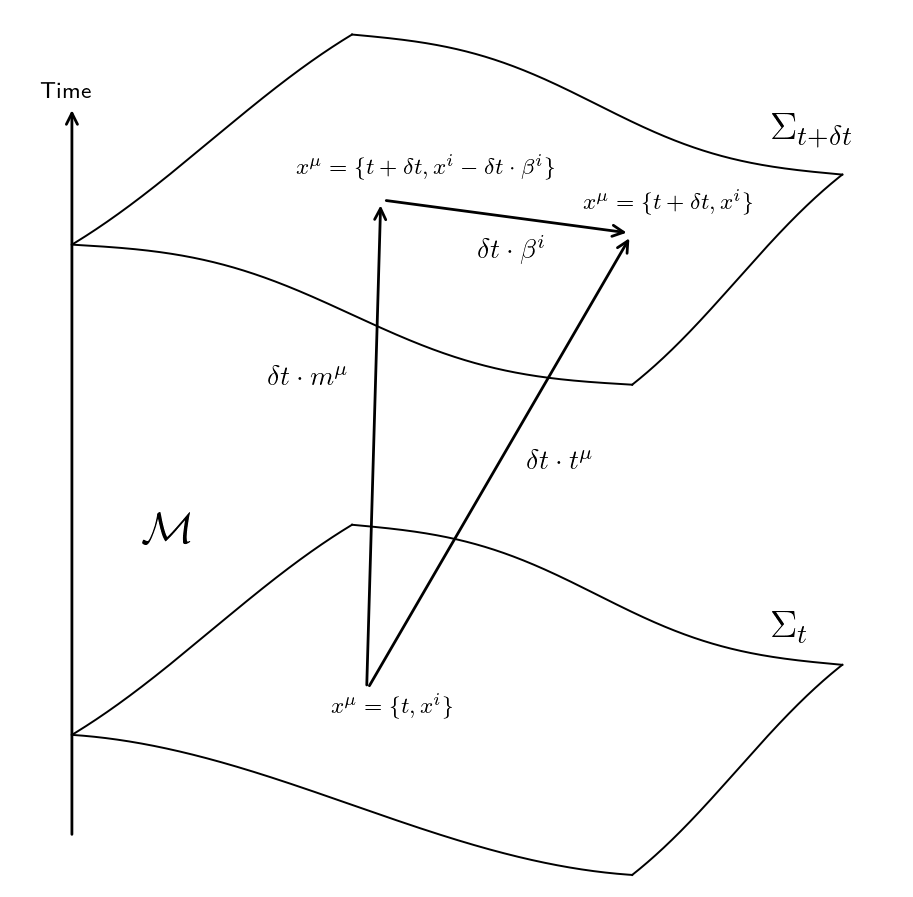
\includegraphics[width=0.65\textwidth]{png/ADM_screeny.png}
    \caption{An illustration of two hypersurfaces $\Sigma_t$ and $\Sigma_{t+\delta}$ and how they are connected by $m^\mu$. As can be seen, integral curves of $t^\mu$ have constant spatial coordinates $x^i$.  }
\end{figure}
\color{orchid} There is a large gauge freedom associated with picking coordinates in general relativity; we choose to use a level set of the time coordinate $x^0=t$ to define our foliation hypersurfaces $\Sigma_t$. \color{black} The other three coordinates $x^i$ for $i\in[1,2,3]$ can be used to span each hypersurface $\Sigma_t$ however we define. It is conventional to split the normal evolution vector $m^\mu$ into time $t^\mu$ and space parts $\beta^\mu$,
\begin{align}
\label{nr:eq:tmu} t^\mu &= \left( 1,0,0,0\right), \\
\label{nr:eq:betamu} \beta^\mu &= \left( 0,\beta^1,\beta^2,\beta^3\right),
\end{align}
such that,
\begin{align}
\label{nr:eq:m1} m^\mu &= t^\mu - \beta^\mu  = (\partial_0)^\mu - \beta^i (\partial_i)^\mu, \\
\label{nr:eq:m2} m^\mu &= \left( 1,-\beta^1,-\beta^2,-\beta^3\right).
\end{align}
We can view $t^\mu$ as the (not necessarily causal) worldline for a simulation gridpoint, hence we would like to evolve our PDEs along $t^\mu$ on a computer. In other words, integral curves of $t^\mu$ must have constant spatial coordinates on $\Sigma_t$. Equation~(\ref{nr:eq:m2}), along with the definitions $\bs{m} = \alpha \bs{n}$ and $\bs{n}^2=-1$, specifies $n^\mu$ and $n_\mu$,
\begin{align}
n^\mu &=  \frac{1}{\alpha}\left( 1,-\beta^1,-\beta^2,-\beta^3\right),\\
n_\mu &= -\alpha\left( 1,0,0,0\right).
\end{align}
The decomposed metric can be calculated, using the property that $\bs{\beta}$ is tangent to $\Sigma_t$ and orthogonal to $\bs{m}$,
\begin{align}
g_{00} &= \bs{g}(\bs{\partial}_0,\bs{\partial}_0) = \bs{g}(\bs{m} + \beta^i \bs{\partial}_i,\bs{m} + \beta^j\bs{\partial}_j) = \bs{g}(\bs{m},\bs{m}) + \beta^i \beta_j \langle \bs{\partial}_i,{\bs{\mathrm{d}}} \bs{x}^j \rangle = -\alpha^2 + \beta^i \beta_i ,\\
 g_{0i} &= \bs{g} (\bs{\partial}_0,\bs{\partial}_i) =  \bs{g}(\bs{m} + \beta^j \bs{\partial}_j, \bs{\partial}_i) =   \beta^j\bs{g}( \bs{\partial}_j, \bs{\partial}_i) = \beta_i,\\
 g_{ij} &= \bs{g}(\bs{\partial}_i,\bs{\partial}_j) = \bs{\gamma}(\bs{\partial}_i,\bs{\partial}_j) = \gamma_{ij}.
 \end{align}
This is commonly called the $3+1$ Arnowitt-Deser-Misner (ADM) metric and $\alpha$, $\beta^i$ are referred to as the lapse and shift vector in this context. The line element and metric are commonly written as,
\begin{align}
\dd s^2 &= -\alpha^2 \dd t^2 + \gamma_{ij}\left[\dd x^i + \beta^i \dd t\right]\left[\dd x^j + \beta^j \dd t\right],\\
 g_{\mu\nu} &= \begin{pmatrix} -\alpha^2 + \beta^i \beta_i & \beta_i \\ \beta_j & \gamma_{ij} \end{pmatrix},\label{nr:eq:admmetric}\\
  g^{\mu\nu} &= \frac{1}{\alpha^2}\begin{pmatrix} -1  & \beta^i \\ \beta^j & \alpha^2\gamma^{ij} - \beta^i \beta^j \end{pmatrix},
 \end{align}
and using Cramer's rule for metric determinant,
\begin{equation} g^{00} = \frac{\det{\gamma_{ij}}}{\det{g_{\mu\nu}}},\end{equation}
we get the important relationship,
\begin{equation} \sqrt{-g} = \alpha \sqrt{\gamma} ,\label{nr:eq:gay}\end{equation}
where $g$ and $\gamma$ are the determinants of $g_{\mu\nu}$ and $\gamma_{ij}$ respectively.

\subsection{ADM Equations} \label{nr:sec:ADM}
Now that we have some coordinates suitable for the spacetime foliation we can find the Arnowitt-Deser-Misner (ADM) evolution equations for $\K_{ij}$ and $\gamma_{ij}$. First we simplify the Lie derivative $\L_t$ along $t^\mu$ using,
\begin{equation}
\L_t \bs{T} = \partial_t \bs{T},
\end{equation}
for any tensor $\bs{T}$ as $\partial_\nu t^\mu=0$. This can be used to expand the Lie derivative along $m^\mu$,
\begin{equation} \L_m = \L_{t} - \L_\beta  = \partial_t - \L_\beta,\end{equation}
and the ADM equations can be written by substituting $\L_m\rightarrow \partial_t - \L_\beta$ in the normal evolution equations in section \ref{nr:sec:einsteindecomp} for $\bs{\K}$ and $\bs{\gamma}$. The ADM equations are,
\begin{align}
\partial_t \K_{ij} &= \L_\beta \K_{ij}  -\D_j\D_i \alpha + \alpha \left[ \R_{ij} + \K\K_{ij} - 2\K^k_i\K_{kj} + 4\pi \left[ \gamma_{ij}\left[ \S-\rho\right]-2\S_{ij}\right]\right],\\
\partial_t \gamma_{ij} &= \L_\beta \gamma_{ij} - 2\alpha\K_{ij}.\end{align}
Unfortunately, these PDEs turn out to be an ill-posed \color{orchid} initial value problem with typical gauges \color{black} \cite{frittelli2000ill}; this means that the time evolution of these equations does not generally depend smoothly on the initial data.


\subsection{BSSN} \label{nr:sec:bssn}
To tackle the ill-posedness of the ADM equations in section \ref{nr:sec:ADM} we now discuss the Baumgarte-Shapiro-Shibata-Nakamura (BSSN) formalism \cite{Baumgarte:1998te} The first step in BSSN is to decompose the 3-metric into the conformal metric $\tilde{\gamma}_{ij}$ and the conformal factor $\chi$,
\begin{align}
\tilde{\gamma}_{ij} &= \chi \gamma_{ij},\\
 \det{\tilde{\gamma}_{ij}} &= \tilde{\gamma} = \chi^3\gamma = 1,
\end{align}
with the above being the convention used in {\sc GRChombo} described in section \ref{grchombo:sec:grchombo}. Other conventions include factors such as
$\tilde{\gamma}_{ij} = \psi^{-4}\gamma_{ij}$ or $\tilde{\gamma}_{ij} =e^{-\phi}\gamma_{ij}$.
Along with this the extrinsic curvature $\K_{ij}$ is conformally decomposed with $\chi$ and modified to be trace free,
\begin{equation} \tilde{A}_{ij} = \chi\left[ \K_{ij}-\frac{1}{3}\K\gamma_{ij}\right], \end{equation} so that $\tilde{A}_{ij}\gamma^{ij}=0$.
During an evolution the condition $\trace{\tilde{A}_{ij}=0}$ (and sometimes $\tilde{\gamma}=1$) is enforced which is observed to improve numerical stability; it is unclear why this works beyond heuristic arguments. As discussed later in section \ref{nr:sec:gaugeconditions}, the definition of $\chi = \gamma^{-1/3}$ is good for black hole simulations where $\gamma\rightarrow\infty$ but $\chi \rightarrow 0$. For example the isotropic Schwarzschild metric has,
\begin{align}
\gamma &= \left[ 1+ \frac{M}{2r}\right]^{12},\\
\chi &=\left[ \frac{r}{\frac{M}{2} + r}\right]^4.
\end{align}

The next step is to introduce the conformal connection functions as auxiliary variables,
\begin{align}
\tilde{\Upsilon}^i &= \tilde{\gamma}^{jk}\tilde{\Upsilon}^i_{\,\;jk} = -\partial_i \tilde{\gamma}^{ij},\\
 \tilde{\Upsilon}^i_{\,\;jk} &= \frac{1}{2}\tilde{\gamma}^{il}\left[ \partial_j \tilde{\gamma}_{kl} + \partial_k \tilde{\gamma}_{lj} - \partial_l \tilde{\gamma}_{jk}\right] = \Upsilon^i_{\;\,jk} + \left[ \delta^i_j \partial_k + \delta^i_k \partial_j - \gamma^{il}\gamma_{jk}\partial_l\right] \ln \sqrt{\chi},
 \end{align}
where $\Gamma^i_{\,\,\,jk}$ are the Christoffel symbols of $\Sigma_t$ as shown in Eq.~(\ref{nr:eq:3connection}).
This reduces the set of vacuum evolution variables to $\{\chi,\tilde{\gamma}_{ij},\K,\tilde{\A}_{ij},\tilde{\Upsilon}^i \}$. It is conventional to use $-\partial_i \tilde{\gamma}^{ij}$ to evaluate the conformal connection coefficients when they appear in the RHS of an equation, but $\partial_j \tilde{\Upsilon}^i$ is calculated by differentiating the evolution variable $\tilde{\Upsilon}^i$. One final necessity, not included in the CCZ4 \color{orchid} (or Z4) \color{black} formulation discussed later, is to add multiples of the constraint equations (in section \ref{nr:sec:einsteindecomp}) to the evolution equations to change the characteristic matrix and improve stability.

The BSSN formalism is not the only way to find a well-posed set of evolution equations for general relativity. Another strongly hyperbolic formalism is the generalised harmonic gauge \cite{Garfinkle:2001ni} \cite{garfinkle2002harmonic} \cite{Pretorius:2004jg} \cite{Pretorius:2005gq} with,
\begin{equation}\Box x^\mu = H^\mu,\end{equation}
for some functions $H^\mu$.


\subsection{Z4 Formalism}
The Z4 formalism \cite{gundlach2005constraint} generalises the Einstein equation to include an unphysical field $Z_\mu$, along with damping terms parameterised by $\kappa_1$, $\kappa_2$,
\begin{equation}\label{nr:eq:z4einstein} R_{\mu\nu} + \nabla_\mu Z_\nu + \nabla_\nu Z_\mu - \kappa_1\left[ n_\mu Z_\nu + n_\nu Z_\mu - [1+\kappa_2]g_{\mu\nu}n^\alpha Z_\alpha\right] = 8\pi G \left[T_{\mu\nu}- \frac{1}{2}Tg_{\mu\nu} \right].\end{equation}
Of course regular General Relativity is recovered by setting $Z_\mu=0$. It can be shown that achieving $Z_\mu=0$ whilst dynamically evolving $Z_\mu$  is equivalent to solving the constraints. $Z_\mu$ is subjected to a wave equation, transporting constraint violation off the computational domain. It can be shown that the system is driven to $Z_\mu =0$ for $k_1>0$ and $k_2>-1$. It is much cheaper to evolve the variables $Z_\mu$, driven to zero, than to solve four elliptic PDEs for the constraints $\{\mathcal{H},\M^i\}$ on each timestep.


\subsection{CCZ4} \label{nr:sec:ccz4}
Merging the conformal decomposition of the BSSN formalism with the constraint damping Z4 formalism gives the conformal covariant Z4 (CCZ4) formalism. The additional modifications,
\begin{align} \Theta &= -n\cdot Z  = -\alpha Z^0,\\
\hat{\Upsilon}^i &= \tilde{\Upsilon}^i + \frac{2\gamma^{ij}Z_j}{\chi},\end{align}
are made, leaving us with the following set of vacuum evolution variables $\{\chi, \tilde{\gamma}_{ij},\K,\tilde{\A}_{ij},\hat{\Upsilon}^i,\Theta \}$. Notably the pair of variables $\R_{ij} + \D_{(i}Z_{j)}$ and its traced version $\R + \bs{\D}\cdot \bs{Z}$, always appear together; separately they would ruin strong hyperbolicity but together they do not. The evolution equations can now be found in the CCZ4 scheme by applying a 3+1 decomposition to the Z4 modified Einstein equation~(\ref{nr:eq:z4einstein}) and proceding as in the BSSN formalism. To illustrate this, we derive the equation of motion for $\chi$ in the CCZ4 formalism. Using Eqs.~(\ref{intro:eq:mdmmdm}) and (\ref{nr:eq:Lmgamma}) with $\chi^{-3}=\gamma$ we obtain,
\begin{align}
\L_m {\gamma} = \gamma \gamma^{ij} \L_m \gamma_{ij} = -2 \gamma \alpha \gamma^{ij} \K_{ij} = -2\gamma \alpha \K.
\end{align}
This can be used to simplify the Lie derivative of $\chi$,
\begin{align}
\L_m \chi &= \L_{\partial_t}\chi - \L_\beta \chi,\\
 &= (\partial_t)^i \partial_i \chi + \omega \chi \partial_i (\partial_t)^i - \beta^i \partial_i \chi - \omega \chi \partial_i \beta^i ,\\
 &= \partial_t \chi - \beta^i \partial_i \chi +\frac{2}{3} \chi\partial_i \beta^i ,\\
\L_m \chi &= \L_m \gamma^{-\frac{1}{3}}  ,\\
&=-\frac{1}{3}\gamma^{-\frac{4}{3}}\L_m \gamma  ,\\
&=\frac{2}{3}\gamma^{-\frac{1}{3}} \alpha \K ,\\
&=\frac{2}{3}\chi\gamma \alpha \K ,
\end{align}
where Eq.~(\ref{intro:eq:Ltensordensity2}) has been used with $\bs{\mathcal{T}}=\chi$ as $\chi$ is a scalar density of weight $\omega=-2/3$. Re-arranging gives the equation of motion for $\chi$,
\begin{equation}
\partial_t \chi =  \beta^i \partial_i \chi + \frac{2\chi}{3} \left[\alpha \K - \partial_i \beta^i \right].
\end{equation}
A similar process returns the remaining CCZ4 equations but care should be taken to include the Z4 terms ($\Theta,\hat{\Upsilon}^i$) where they are needed. The complete list of CCZ4 equations used in simulations with {\sc GRChombo} (section \ref{grchombo:sec:grchombo}) are given below:
\begin{align} \partial_t \chi &=  \beta^i \partial_i \chi + \frac{2\chi}{3} \left[\alpha \K - \partial_i \beta^i \right],\\
\partial_t\tilde{\gamma}_{ij} &=  \beta^k\partial_k\tilde{\gamma}_{ij}  + \tilde{\gamma}_{kj}\partial_i \beta^k + \tilde{\gamma}_{ik}\partial_j\beta^k - \frac{2}{3}\tilde{\gamma}_{ij} \partial_k \beta^k - 2\alpha\tilde{\A}_{ij},\\
\partial_t\K &=  \beta^k\partial_k\K + \alpha\left[ \R + 2\bs{\D}\cdot \bs{Z} + \K\left[ \K-2\Theta\right]\right] - 3\alpha \kappa_1\left[ 1+\kappa_2\right]\Theta \nonumber\\
&-\chi\tilde{\gamma}^{kl}\D_k\D_l\alpha + 4\pi G\alpha\left[ \S - 3\rho\right], \\
\partial_t\tilde{\A}_{ij} &=  \beta^k \partial_k \tilde{\A}_{ij}+\chi\left[\alpha\left[\R_{ij} + 2\D_{(i}Z_{j)}-8\pi G \S_{ij} \right] -\D_i\D_j\alpha \right]^{TF}\nonumber\\
& +\tilde{\A}_{ij}\left[ \alpha\left[ \K-2\Theta\right]-\frac{2}{3}\K^2\right] + 2\tilde{\A}_{k(i}\partial_{j)}\beta^k -2\alpha\tilde{\gamma}^{kl}\tilde{\A}_{ik}\tilde{\A}_{lj},\\
\partial_t\Theta &= \beta^k\partial_k \Theta + \frac{1}{2}\alpha\left[ \R + 2\bs{\D}\cdot \bs{Z} - \tilde{\A}_{kl} \tilde{\A}^{kl} + \frac{2}{3}\K^2 - 2\Theta\K\right] -\kappa_1\alpha\Theta\left[ 2+\kappa_2\right] - Z^k\partial_k\alpha - 8\pi G \alpha \rho, \\
\partial_t\hat{\Upsilon}^i &=  \beta^k \partial_k \hat{\Upsilon}^i + \frac{2}{3}\left[ \partial_k \beta^k \left[ \tilde{\Upsilon}^i+2\kappa_3 \frac{Z^{i}}{\chi}\right]-2\alpha\K\frac{Z^j}{\chi}\right]-2\alpha\kappa_1\frac{Z^i}{\chi}\nonumber \\
& + 2\tilde{\gamma}^{ij}\left[ \alpha\partial_j\Theta -\Theta \partial_j\alpha \right] -2\tilde{\A}^{ij}\partial_j\alpha - \alpha\left[ \frac{4}{3}\tilde{\gamma}^{ij}\partial_j\K + 3\tilde{\A}^{ij}\frac{\partial_j \chi}{\chi}\right]\nonumber\\
& -\left[ \tilde{\Upsilon}^j + 2\kappa_3 \frac{Z^j}{\chi}\right]\partial_j \beta^i + 2\alpha \tilde{\Upsilon}^i_{\,\,\,jk}\tilde{\A}^{jk} + \tilde{\gamma}^{jk}\partial_j\partial_k \beta^i + \frac{1}{3} \tilde{\gamma}^{ij}\partial_k \partial_j \beta^k - 16\pi G \alpha \tilde{\gamma}^{ij}\S_j, \\
\partial_t \vp &= \beta^k\partial_k \vp - \alpha\Pi ,\label{nr:eq:ccz4kg1}.\end{align}
In the CCZ4 equations there is an additional parameter $\kappa_3$ premultiplying terms in the evolution of $\hat{\Upsilon}^i$ which experimentally were found to lead to instabilities in black hole simulations \cite{PhysRevD.85.064040}; setting $\kappa_3<1$ stabilises the simulation but at the cost of covariance. Later on it was realised that setting $\kappa_3=1$ and $\alpha\kappa_1\rightarrow\kappa_1$ retains covariance as well as numerical stability \cite{Alic:2013xsa}; in this work $\kappa_1=0.1$, $\kappa_2=0$ and $\kappa_3=1$ is used.


The CCZ4 scheme proves several benefits.
\begin{itemize}
\item Any initial data that does not satisfy the constraints will generally not do so during evolution when using the BSSN formalism either. Given that superposition of solutions in GR does not generally give a new solution, but does approximate one for separated compact objects, all the simulated binaries considered in this work will have non constraint satisfying initial data.
\item Constraint satisfying initial data can also develop constraint violation over time; one reason being that finite resolution imposes some small deviation from the continuum solution. More importantly, the use of adaptive mesh refinement (discussed in section \ref{grchombo:sec:grchombo}) introduces interpolation errors into the simulation at the boundary of the different grid resolution levels. The use of the CCZ4 scheme can also help to reduce the constraint violation generated in this way.
\item Sommerfeld boundary conditions (discussed in section \ref{grchombo:sec:sommerfeld}) used are inexact in GR and will introduce errors at the outer boundary that ruin constraint satisfaction. \color{gren} sommerfeld are ill posed? \color{black}
\end{itemize}
In all the cases above, the CCZ4 system forces the evolution towards constraint satisfaction, despite the numerical errors and approximations. There is a caveat, even if a simulation satisfies the constraints, there is no guarantee it is the desired solution to Einstein's equation. \color{orchid} Additionally, the damping is more efficient for small amplitude and high frequency erorrs. \color{black}



\subsection{Gauge Conditions}\label{nr:sec:gaugeconditions}

\color{gren} PUT A FEW BOOK CITATIONS IN HERE! \color{black}

The lapse $\alpha$ and shift $\beta^i$ are freely specifiable on a hypersurface $\Sigma_t$ being gauge variables, however they must be chosen carefully along with a suitable initial Cauchy surface $\Sigma_{t_0}$ and initial data. $\Sigma_{t_0}$ should be a smooth non-intersecting Cauchy surface as described in section \ref{nr:sec:foliation} and contain smooth initial data. It is also wise to avoid singularities (both coordinate and physical) on this surface. As an example, consider the simulation of a single Schwarzschild black hole. Figure~\ref{nr:fig:eddington-finkelstein} (left) shows how an initial data surface could extend to the singularity if polar-areal coordinates are used. Figure~\ref{nr:fig:eddington-finkelstein} also shows how the physical singularity is avoided when using isotropic coordinates. In this work the isotropic gauge is used; not only does this provide an initial Cauchy surface free of physical singularities but also allows for trivial swapping between spherical polar and Cartesian (used in simulations) coordinates. However, for a poor choice of lapse function, even a well chosen $\Sigma_{t_0}$ can advance to the physical singularity in finite simulation time.

%   \begin{figure}[h]
%   \caption{Penrose Diagrams, $\Sigma_{t_0}$ dashed, Left: Ingoing Eddington-Finkelstein Coordinates, Right: Isotropic Coordinates.}
%   \centering
%   \subfloat{\includegraphics[width=0.43\textwidth]{schwarzschild2.png}\label{boson:fig:f1}} \label{nr:fig:eddington-finkelstein}
%   \hfill
%   \subfloat{\includegraphics[width=0.5\textwidth]{schwarzschild.png}\label{boson:fig:f2}} \label{nr:fig:isotropic}
% \end{figure}

  \begin{figure}[h]
  \caption{Penrose Diagram of the maximally extended Schwarzschild spacetime; the top (future) squiggle represents the spacelike black hole singulary and the bottom (past) squiggle represents the white hole singularity. In the right hand diagram, the straight dashed line labelled by $\Sigma_{\rm iso}$ represent the initial hypersurface $\Sigma_{t_0}$ for $t=0$ in isotropic coordinates. In the left hand diagram, the dashed line labelled by $\Sigma_{\rm pa}$ represent the initial hypersurface $\Sigma_{t_0}$ for $t=0$ in polar-areal coordinates. Notably $\Sigma_{\rm pa}$ initially touches the physical singularity whereas $\Sigma_{t_0}$ does not; additionally $\Sigma_{\rm pa}$ is not a Cauchy surface as there exist causal curves which can intersect it multiple times.}
  \centering
  \subfloat{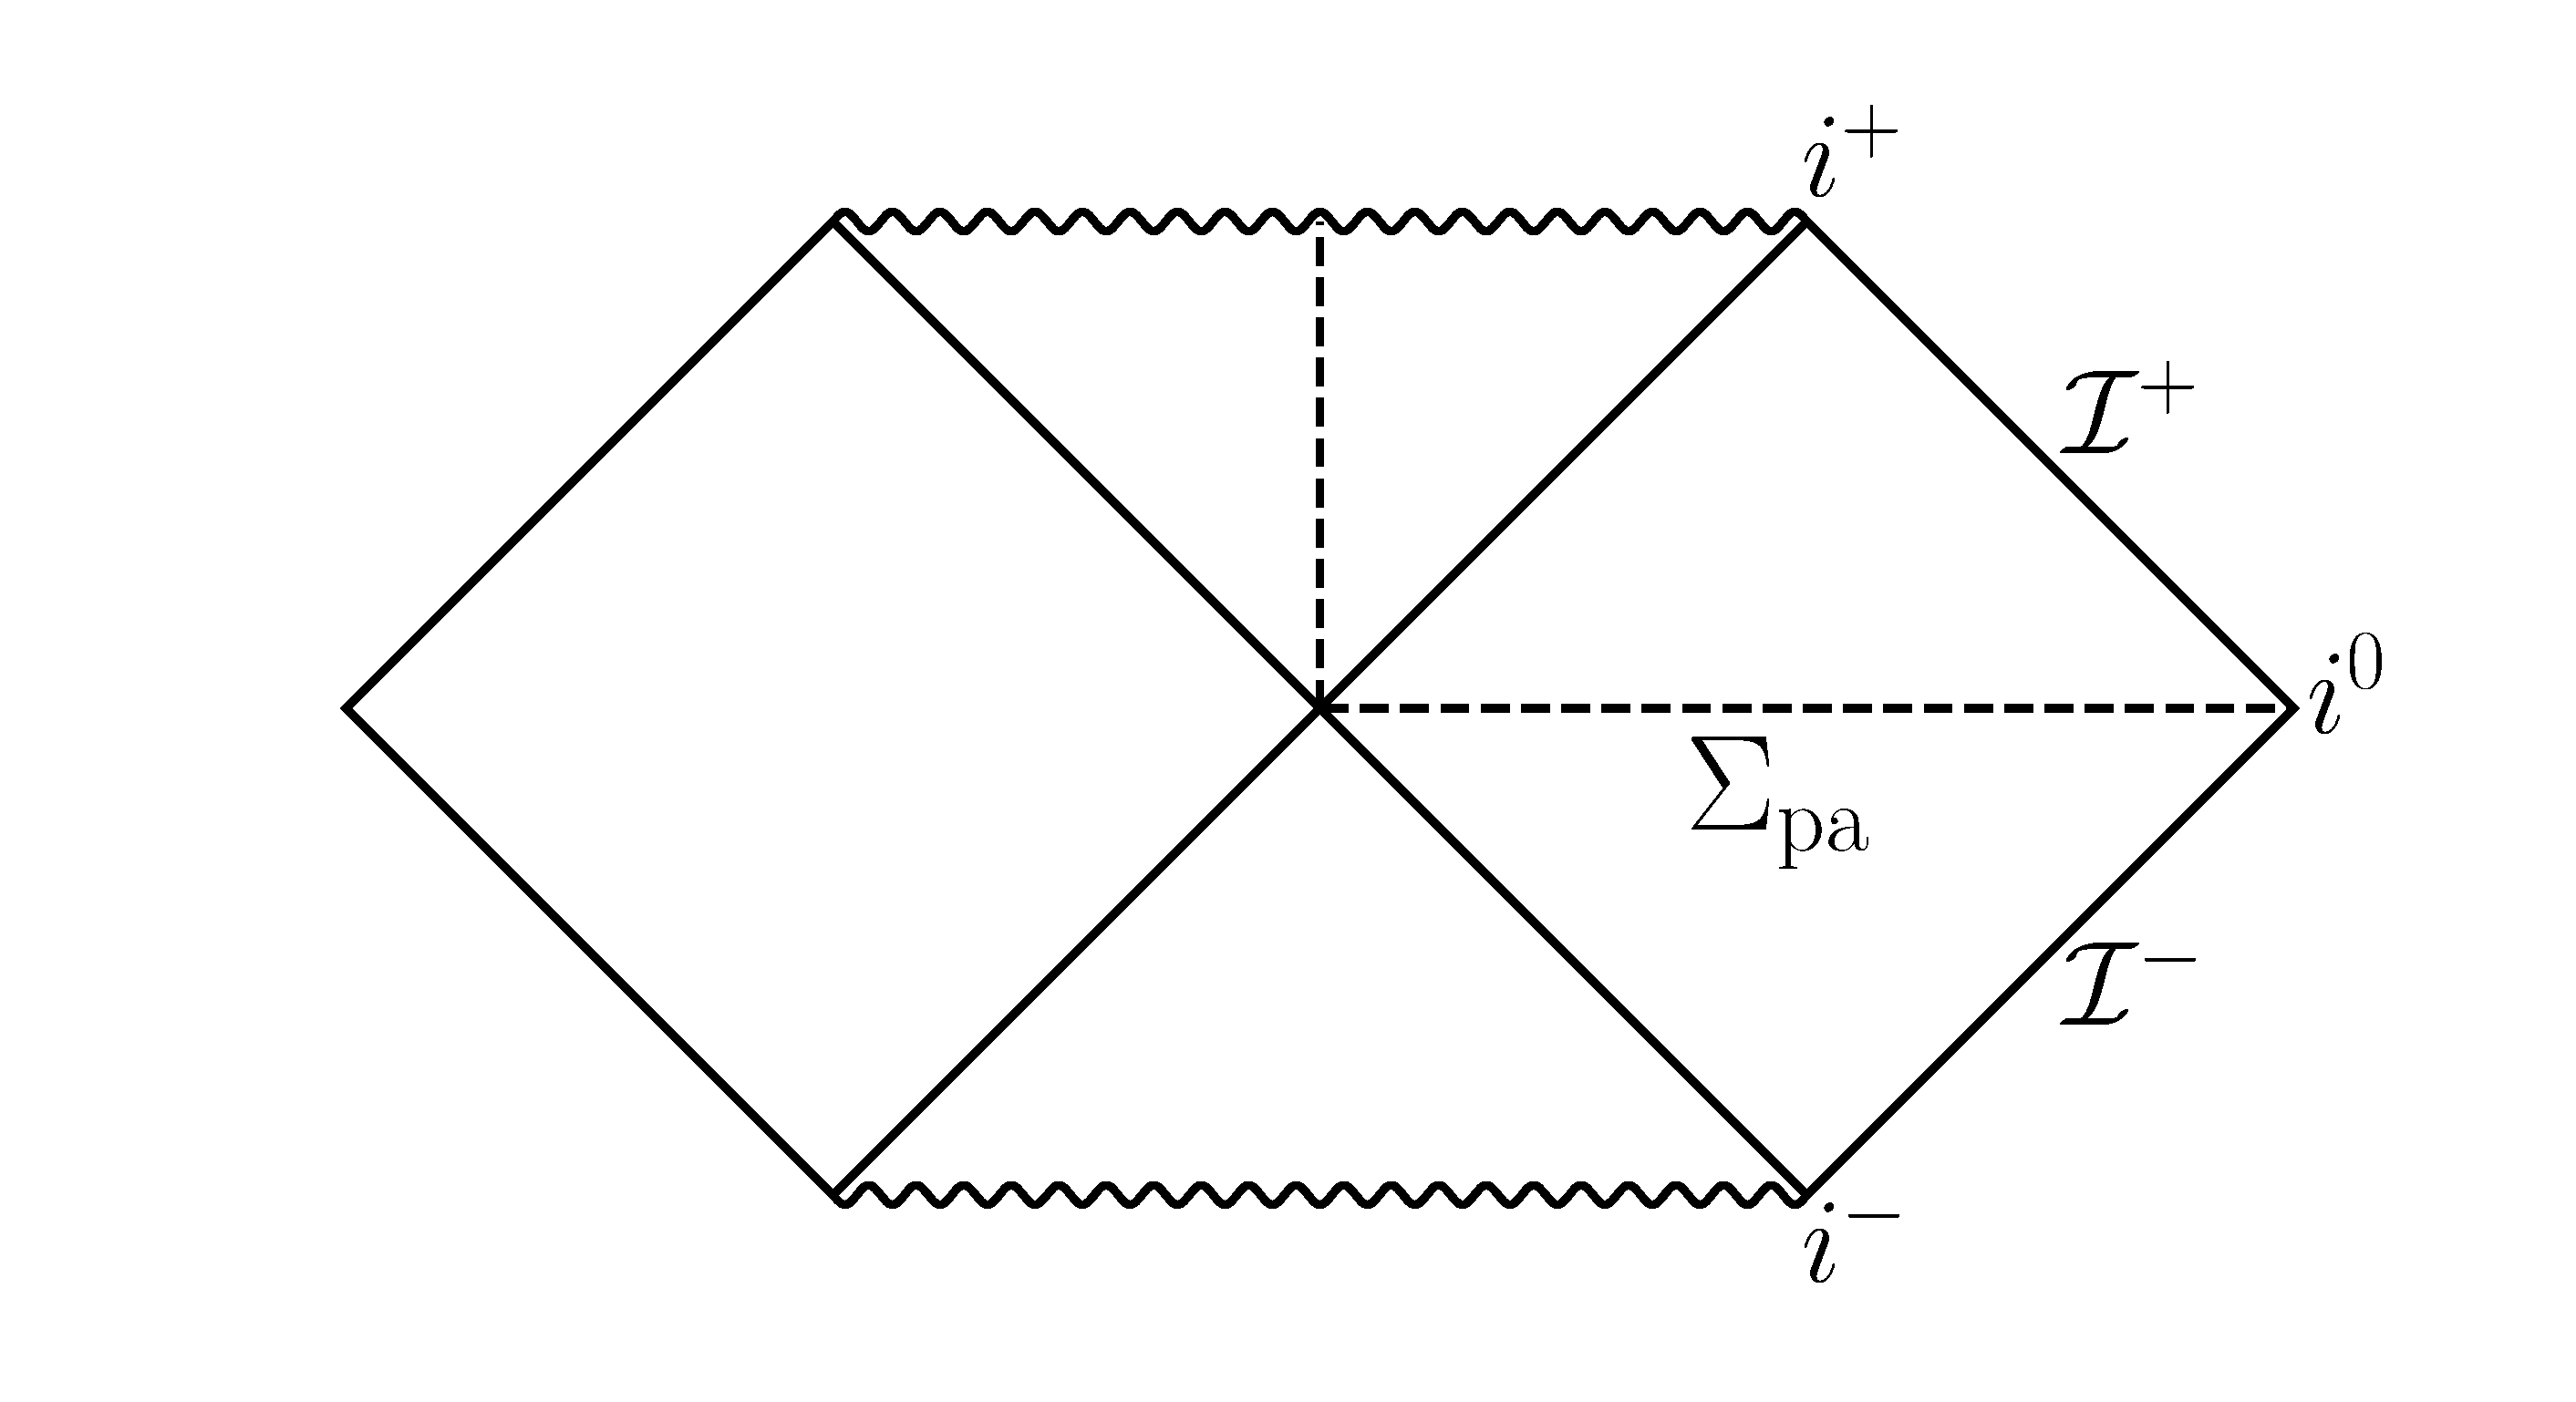
\includegraphics[width=0.50\textwidth]{png/penrose_sc.pdf}} \hfill
  \subfloat{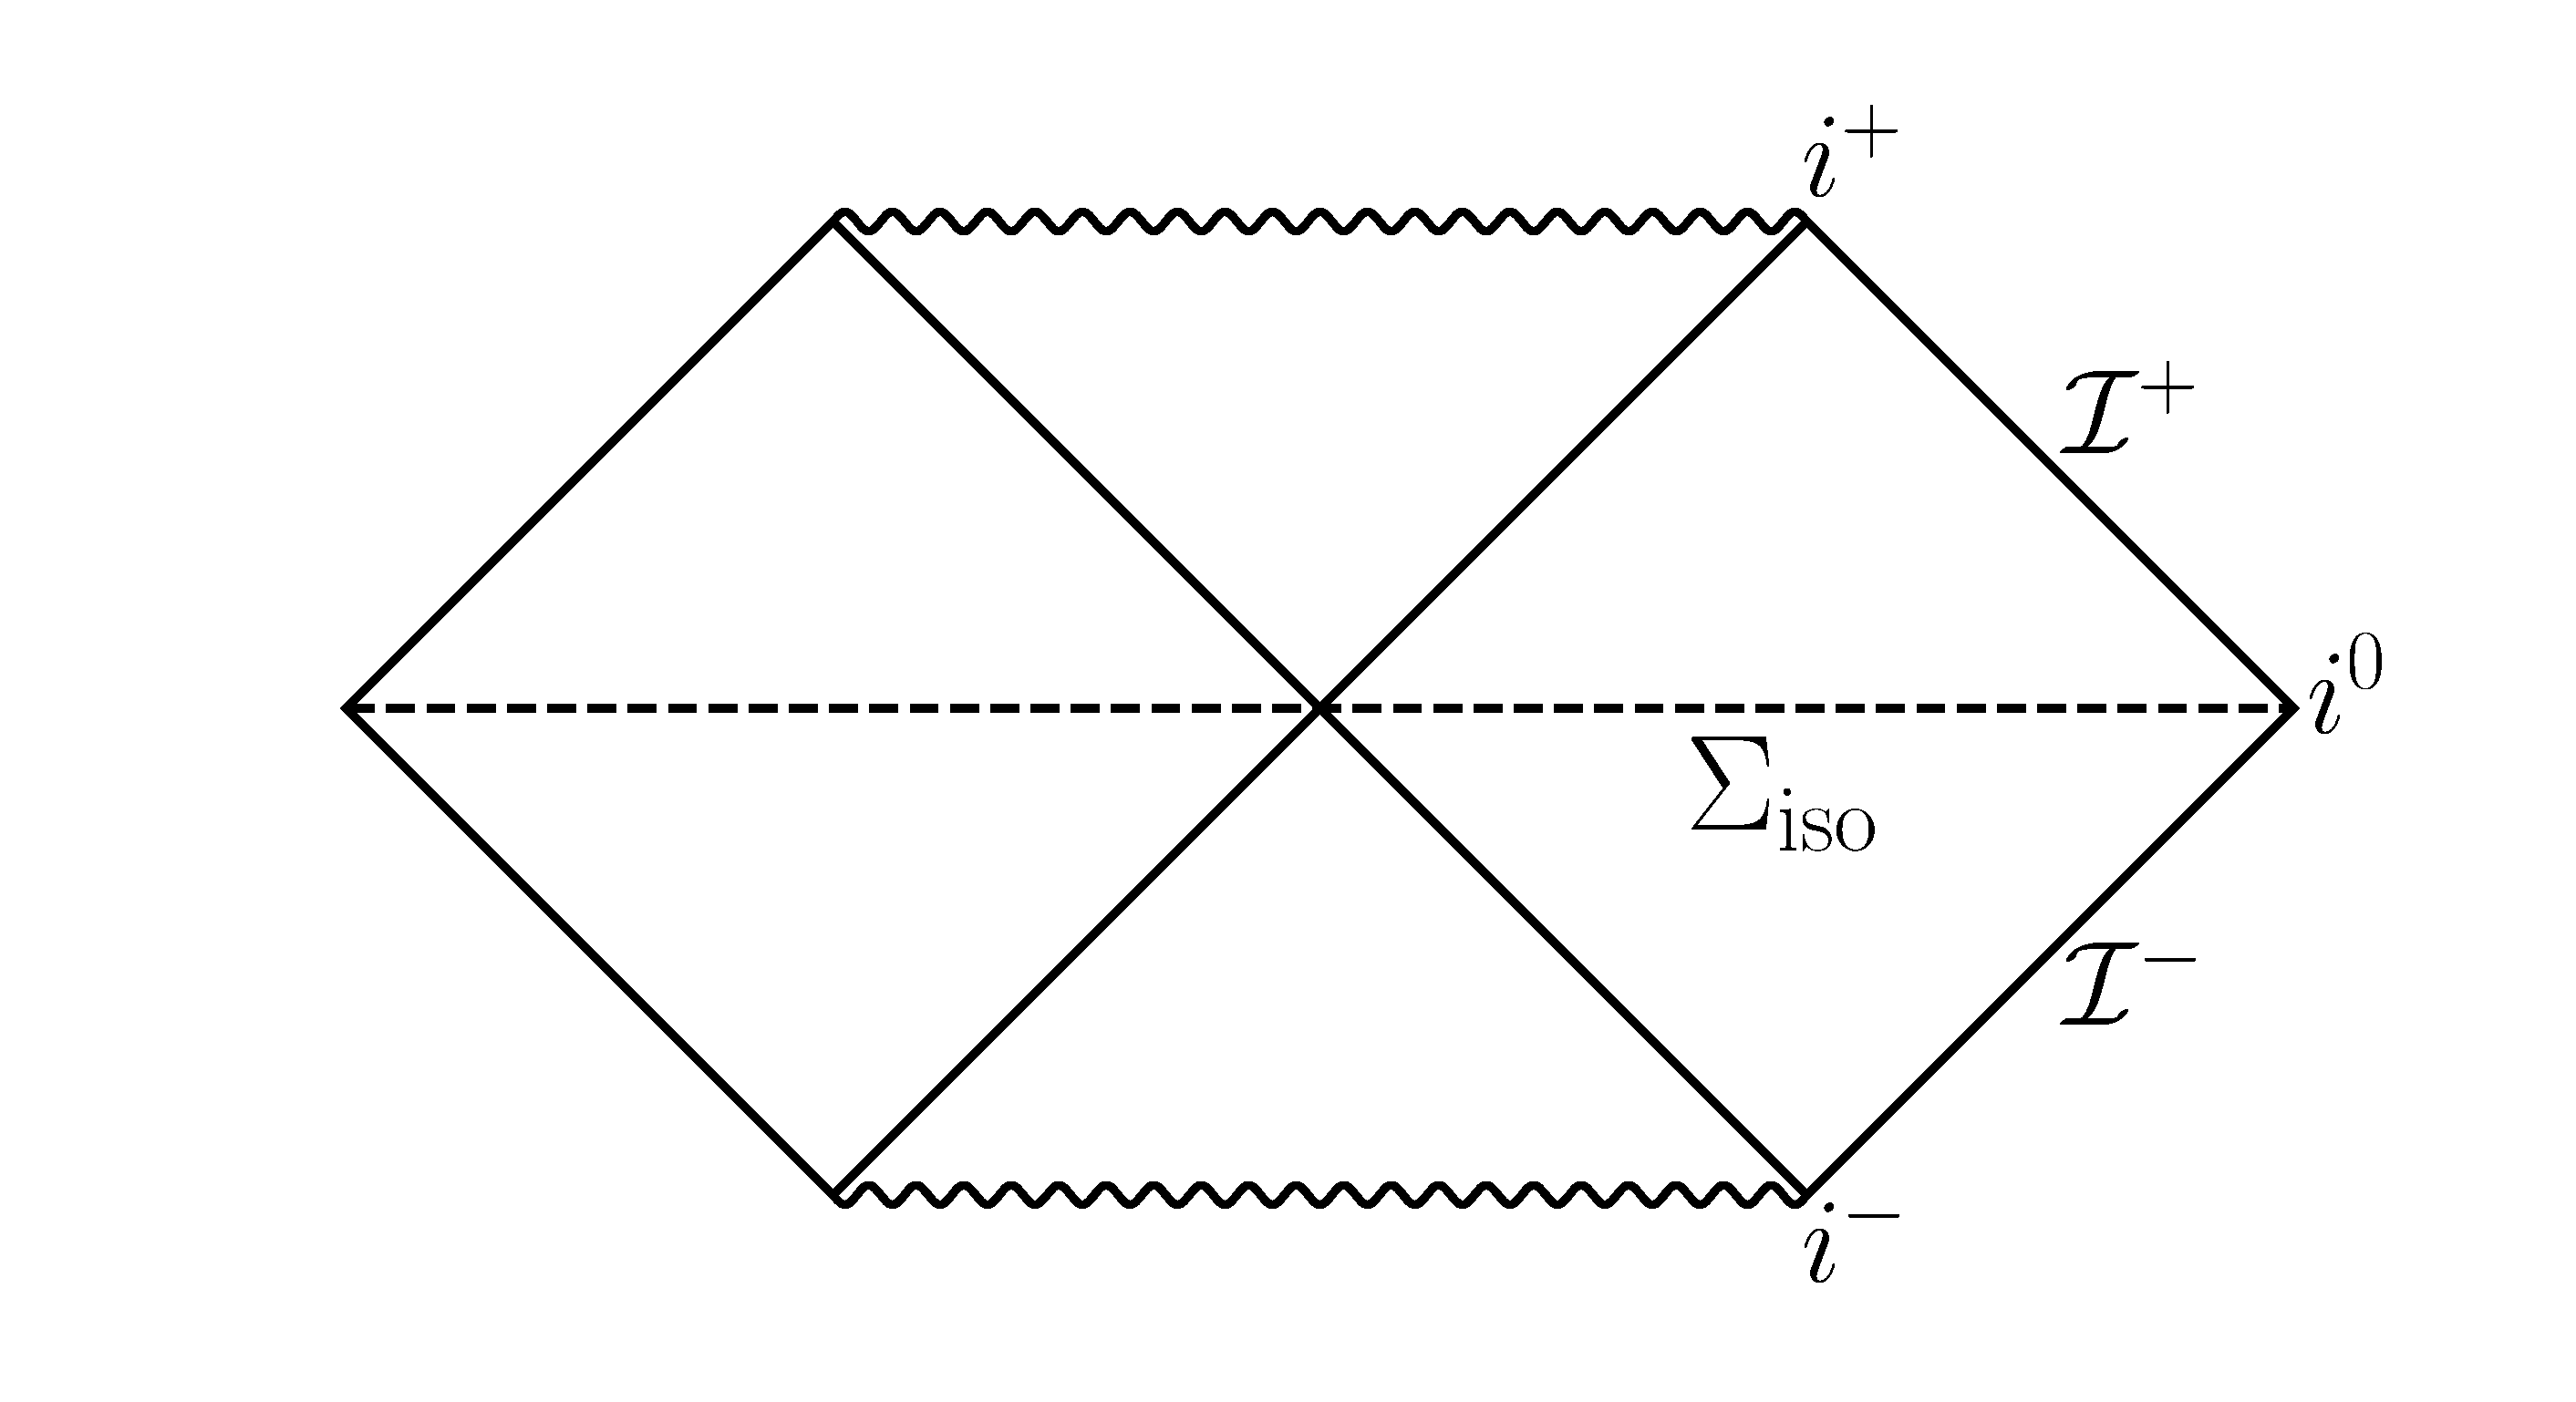
\includegraphics[width=0.50\textwidth]{png/penrose_iso.pdf}}
  \label{nr:fig:eddington-finkelstein}\label{nr:fig:isotropic}\label{boson:fig:f1}
\end{figure}

\subsubsection{Lapse Slicing Conditions}

The simplest lapse choice would be to enforce $\alpha=1$, called geodesic slicing, with the hypersurface following integral curves of $n^\mu$; given that geodesics can converge this can lead to hypersurface self-intersection which breaks the definition of a Cauchy surface and the simulation will likely fail. Another problem is that a black hole singularity can be reached in finite simulation time.

An alternative slicing condition is the maximal slicing condition which keeps the volume element $\sqrt{-g}$ constant along geodesics. This means as $\gamma\rightarrow\infty$ nearing a singularity $\alpha\rightarrow0$ from Eq.~(\ref{nr:eq:gay}), causing the hypersurface to advance more slowly before a singularity is reached as demonstrated in Fig.~(\ref{nr:fig:singularity_avoiding}). This property is called singularity avoiding and is crucial for numerical stability unless using excision\footnote{Excision is the practice of cutting singularities out of the computational domain while supplying suitable boundary conditions about the excised region}. Maximal slicing can be implemented by forcing $\mathcal{K} = \partial_t \K = 0\,\forall \,t$ which requires a slow elliptic solve for $\alpha$ at each timestep. Instead of performing this slow elliptic solve, $\alpha$ is promoted to an evolution variable and is evolved along with every other simulation variable. To do this we can pick an algebraic slicing condition of the Bona-Masso type,
\begin{equation}\L_m \alpha = \partial_t \alpha - \beta^i \partial_i \alpha = -\alpha^2 f(\alpha)\K. \end{equation}
Using this with $f = 2\alpha^{-1}$ gives,
\begin{equation}\L_m \alpha = \partial_t \alpha - \beta^i \partial_i \alpha = -2\alpha \K, \label{nr:eq:1pluslog} \end{equation}
which is called 1+log slicing; this is very common in Numerical Relativity codes. In practice 1+log slicing is strongly singularity avoiding reaching $\alpha=0$ before the singularity. This is modified in the CCZ4 scheme to,
\begin{equation}\partial_t \alpha = -2\alpha\left[ \K-2\Theta\right] + \beta^i \partial_i \alpha.\end{equation}
Using Gaussian normal coordinates $\beta^i=0$ and provided $\Theta=0$, the 1+log slicing condition reduces to,
\begin{equation} \alpha = 1+ \ln \gamma,\end{equation}
giving the slicing condition it's name \cite{alcubierre2008introduction}.

\begin{figure}[h!]
    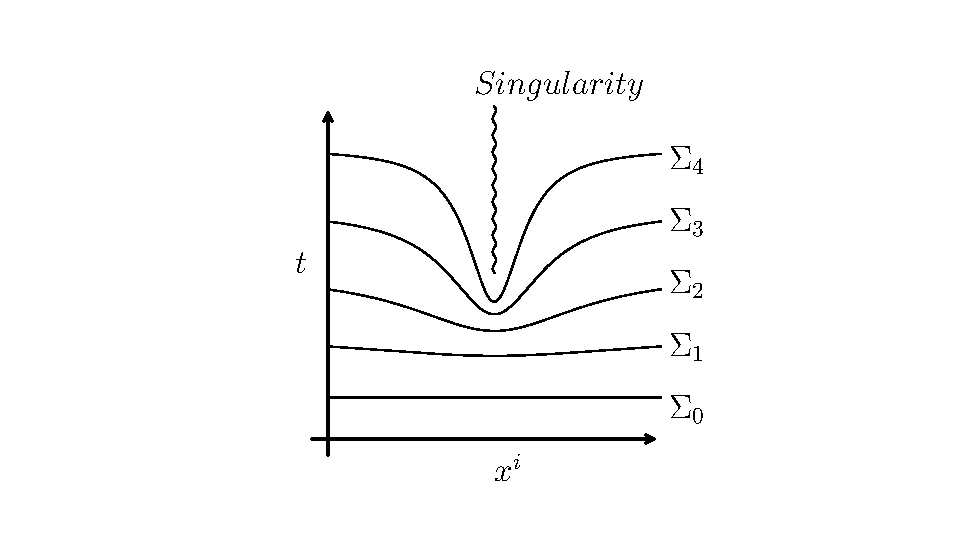
\includegraphics[width=0.9\textwidth]{png/slicing.pdf}
      \caption{Diagram showing the time evolution of a hypersurface using a singularity avoiding slicing condition. The vertical squiggled line represents a physical singularity that is formed at some point in spacetime, potentially from the collapse of matter to a black hole.} \label{nr:fig:singularity_avoiding}
\end{figure}


\subsubsection{Shift Conditions}

The simplest choice for the shift vector would be $\beta^i=0$ but this can cause great stretching and shearing of integral curves of $m^\mu$ in the neighbourhood of a singularity as in Fig.~(\ref{nr:fig:singularity_avoiding}); the effect of this is that neighbouring gridpoints may have large differences in field values leading to inaccurate and unstable evolutions.

 Another negative side effect is that the computational domain can fall inside an event horizon in black hole simulations. To counteract this we want to employ a shift vector that minimises hypersurface shear $\sigma_{ij}$ which can be defined as \cite{smarr1978kinematical},
\begin{equation} \sigma_{ij}:= \perp^\mu_i \perp^\nu_j \left[\nabla_{(\mu} n_{\nu)}-\frac{1}{3}\gamma^{ab}\nabla_{(a} n_{b)} \gamma_{\mu\nu}\right], \end{equation}
where $\sigma_{ij}$ is tracefree corresponding to shearing rather than inflation or expansion. Minimising the total shear $\Sigma$,
\begin{equation} \Sigma = \int \sigma_{ij}\sigma^{ij}\sqrt{\gamma}\,\dd x^3,\end{equation}
with respect to $\beta^i$ leads to an elliptic PDE to be solved for each $\beta^i$ at each time step that minimises shear,
\begin{equation} \delta \Sigma = 0 \rightarrow \D_i\sigma^{ij}=0.\end{equation}
This is known as the minimal distortion shift condition. Promoting the $\beta^i$ to evolution variables is computationally cheaper than solving a set of PDEs at each time step. A very common choice is to promote the elliptic PDE for $\beta^i$ into a hyperbolic equation via introducing a $\partial_t^2\beta^i$ term and an artificial damping term parameterised by $\eta$. This becomes a damped wave equation and is supposed to transport away any part of $\beta^i$ which does not satisfy $\D_i \sigma^{ij}=0$. This works well with Sommerfeld (outgoing wave) boundary conditions given in section \ref{grchombo:sec:sommerfeld}. The standard Gamma driver shift condition is,
\begin{align}
\partial_t \beta^i &= FB^i,\label{nr:eq:gammadriver1}\\
 \partial_t B^i &= \partial_t \tilde{\Gamma}^i - \eta B^i,\label{nr:eq:gammadriver2}\end{align}
where $F=3/4$ and $\eta=1$ are used throughout this work.

\subsubsection{Moving Puncture Gauge}
The moving puncture gauge (MPG) is the combination of the 1+log slicing lapse condition
in Eq.~(\ref{nr:eq:1pluslog}) and the Gamma driver shift condition in
Eqs.~(\ref{nr:eq:gammadriver1}) and (\ref{nr:eq:gammadriver2}). In 2006, the
moving puncture gauge allowed for the first successful simulation of a black hole
binary \cite{PhysRevLett.96.111101} in the \color{orchid} BSSN \color{black}
formalism\footnote{It should be noted that a black-hole binary had been sucessfully
simulated before by \cite{Bruegmann:2003aw} in 2003 with co-rotating coordinates
and \cite{Pretorius:2005gq} in 2005 using the generalised harmonic gauge.} without
the use of excision. \color{gren} maybe david/others deserve a citation here for
z4c/ccz4. \color{black} Even though $\chi\rightarrow 0$, or $\gamma \rightarrow \infty$,
at the centre of a black hole, as long as a minimum value for $\chi$
(such as $\chi=10^{-4}$) is enforced a simulation can run. \color{orchid} Even though it is
unphysical to modify a physical variable, the success of the MPG is often attributed
to the causal shielding\footnote{\color{orchid} Errors that propagate at (or below) light speed
will be trapped by the event horizon. } provided by the
event horizon. Additionally, any extremely sharp field configurations produced will
be partially suppressed by a numerical dissipation scheme.\color{black}

Not only does the MPG safeguard the divergence of fields at the puncture, but it allows the puncture to move; hence the name {\it moving} puncture gauge. Near the puncture, the lapse $\alpha$ becomes vanishingly small and the 1+log slicing condition in Eq.~(\ref{nr:eq:1pluslog}) becomes,
\begin{equation}
\partial_t \alpha = \beta^i \partial_i \alpha, \label{nr:eq:betavel}
\end{equation}
which causes the puncture to move. Assigning spatial coordinates $x^i_{\rm punc}(t)$ to the puncture, we know that
\begin{align}
\alpha(x^i_{\rm punc}) &= 0,\\
\frac{\dd}{\dd t} \alpha(x^i_{\rm punc})  &= \frac{\partial}{\partial t}\alpha + \left(\frac{\partial x^i}{\partial t}\Bigg|_{x^i=x^i_{\rm punc}}\right)\frac{\partial}{\partial x^i} \alpha =0,
\end{align}
which can be compared to Eq.~(\ref{nr:eq:betavel}) to show that
\begin{equation}
\beta^i = -\frac{\partial }{\partial t}x^i_{\rm punc}\,.
\end{equation}
This shows that the puncture must move along integral curves of $-\beta^i$.
